\documentclass[10pt,a4paper]{article}
\usepackage[utf8]{inputenc}
\usepackage{amsmath}
\usepackage{amsfonts}
\usepackage{amssymb}
\usepackage{dsfont}
\usepackage{graphicx}
\newcommand{\norm}[1]{\left\lVert#1\right\rVert}
\title{cs234 hw3}
\date{2022-01-23}
\author{Jon Sondag}
\setcounter{section}{0}
\begin{document}
  \maketitle
  \section{Policy Gradient Methods}
  \setcounter{subsection}{4}  
  \subsection{}
  \paragraph{(a)(i)}
  Cartpole with baseline, $r\_seed=15$: \\
  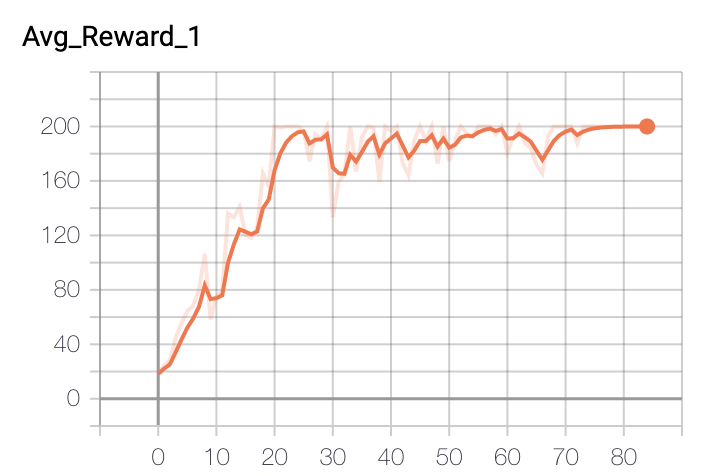
\includegraphics[scale=0.5]{images/cartpole_baseline_15_avg_reward.png} \\
  Cartpole no baseline, $r\_seed=15$: \\
  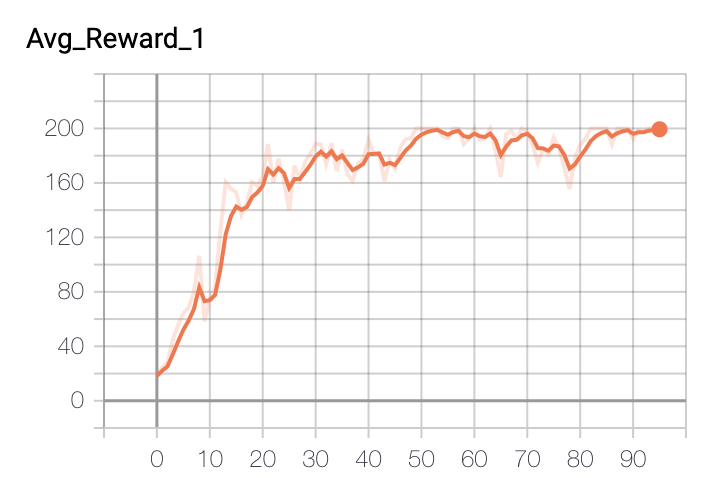
\includegraphics[scale=0.5]{images/cartpole_nobaseline_15_avg_reward.png} \\
  There's not a significant difference between the two reward graphs.
  \paragraph{(a)(ii)}
  Cartpole with baseline, $r\_seed=12345456$: \\  
  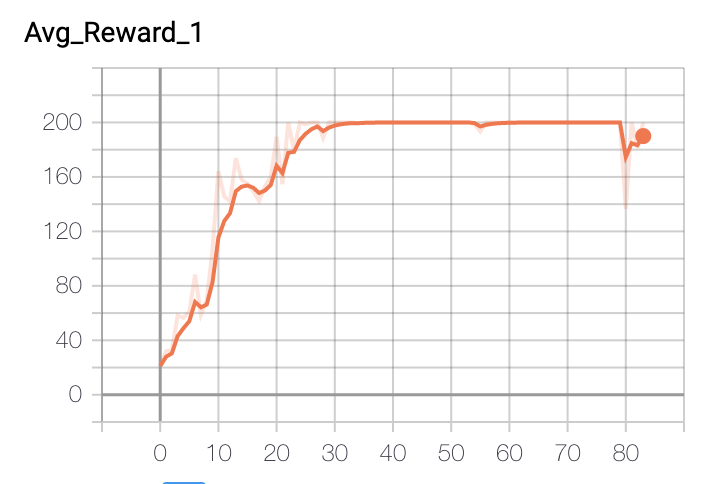
\includegraphics[scale=0.5]{images/cartpole_baseline_12345456_avg_reward.png} \\  
  Cartpole no baseline, $r\_seed=12345456$: \\  
  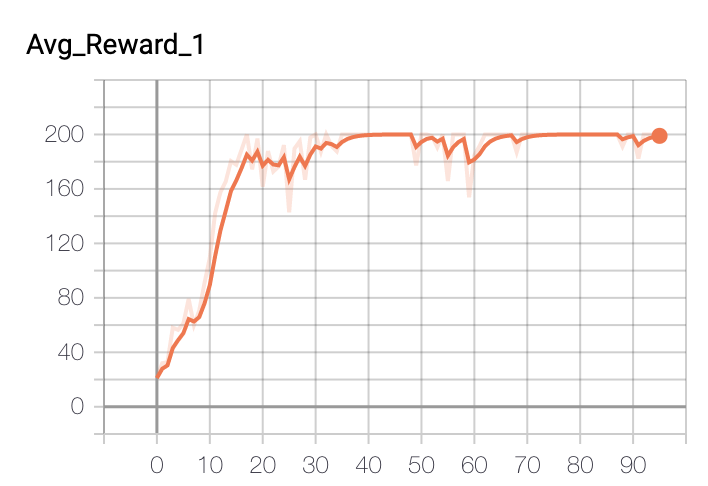
\includegraphics[scale=0.5]{images/cartpole_nobaseline_12345456_avg_reward.png} \\    
  The no baseline reward chart shows slightly more wiggle but this may just be due to noise. 
  \paragraph{(b)(i)}  
  Pendulum with baseline, $r\_seed=15$: \\
  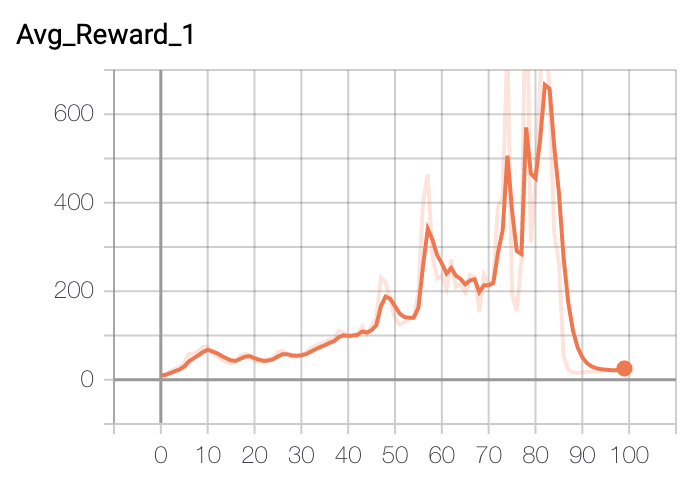
\includegraphics[scale=0.5]{images/pendulum_baseline_15_avg_reward.png} \\
  Pendulum no baseline, $r\_seed=15$: \\
  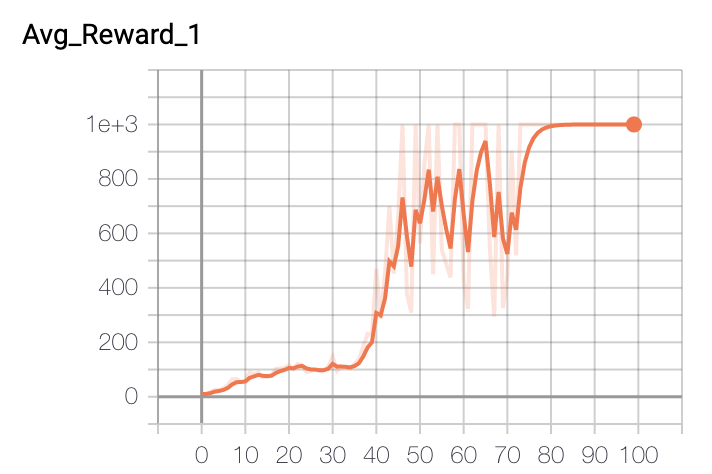
\includegraphics[scale=0.5]{images/pendulum_nobaseline_15_avg_reward.png} \\
  The no baseline reward ends at the maximum reward for the last 20+ batches.  The baseline reward ends up going down significantly over the last 10-20 batches.  The baseline reward also takes longer to achieve the maximum reward, maybe in part due to its lower variance.
  \paragraph{(b)(ii)}    
  Pendulum with baseline, $r\_seed=8$: \\
  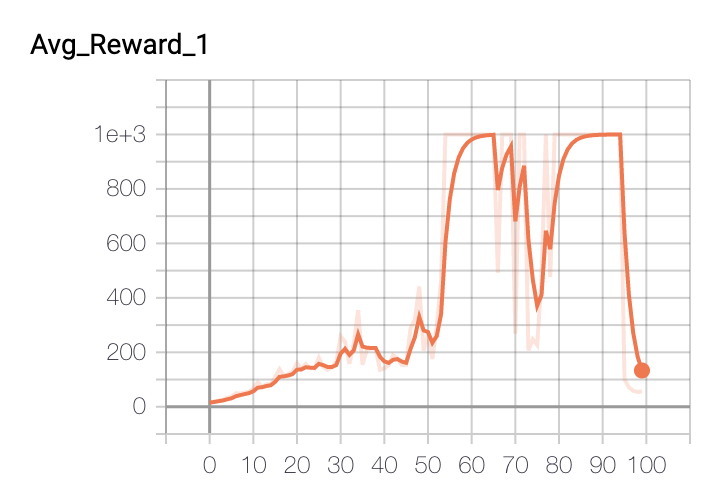
\includegraphics[scale=0.5]{images/pendulum_baseline_8_avg_reward.png} \\
  Pendulum no baseline, $r\_seed=8$: \\
  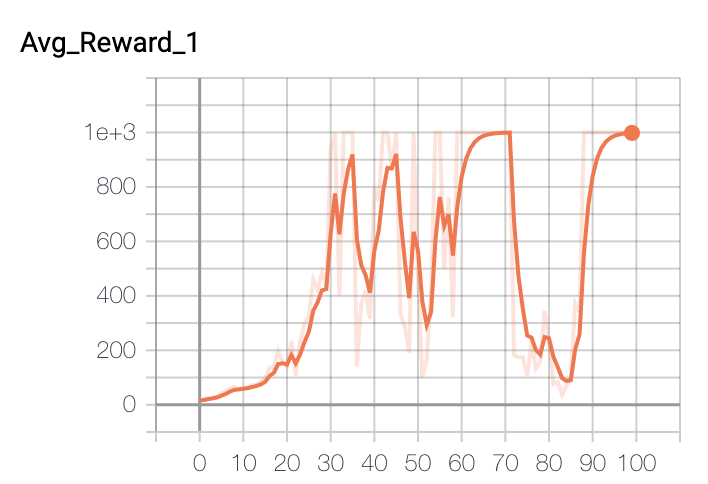
\includegraphics[scale=0.5]{images/pendulum_nobaseline_8_avg_reward.png} \\
  Again with this seed, the baseline reward takes longer to achieve the maximum reward, maybe in part due to its lower variance.
  \paragraph{(c)(i)}  
  Cheetah with baseline, $r\_seed=123$: \\
  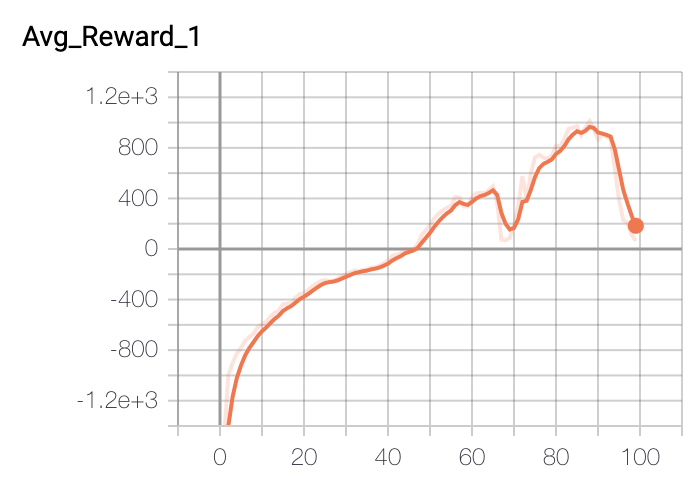
\includegraphics[scale=0.5]{images/cheetah_baseline_123_avg_reward.png} \\
  Cheetah no baseline, $r\_seed=123$: \\
  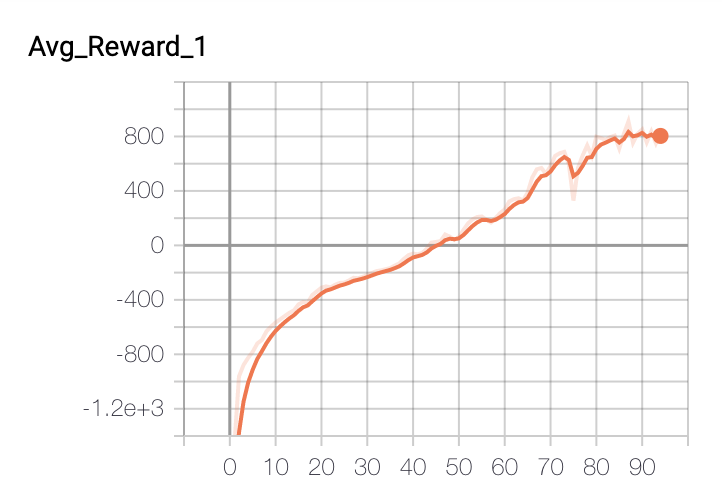
\includegraphics[scale=0.5]{images/cheetah_nobaseline_123_avg_reward.png} \\
  Surprisingly, the no baseline case has lower variance.
  \paragraph{(c)(ii)}    
  Cheetah with baseline, $r\_seed=15$: \\
  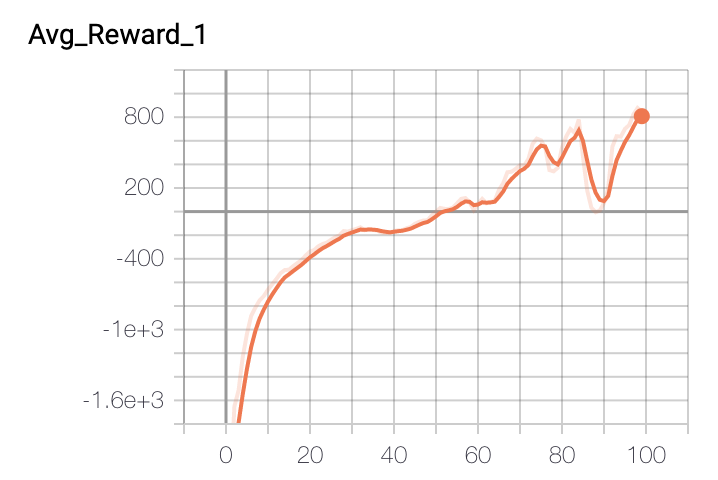
\includegraphics[scale=0.5]{images/cheetah_baseline_15_avg_reward.png} \\
  Cheetah no baseline, $r\_seed=15$: \\
  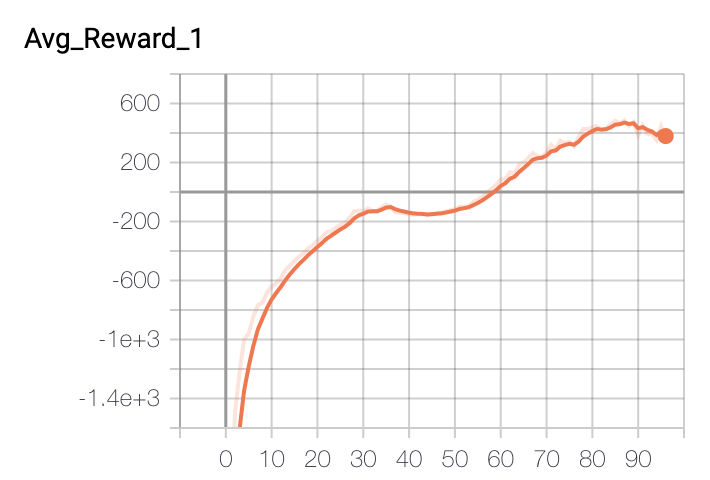
\includegraphics[scale=0.5]{images/cheetah_nobaseline_15_avg_reward.png} \\
  Surprisingly, the no baseline case has lower variance.  
  \paragraph{(c)(iii)}    
  Cheetah with baseline, $r\_seed=12345456$: \\
  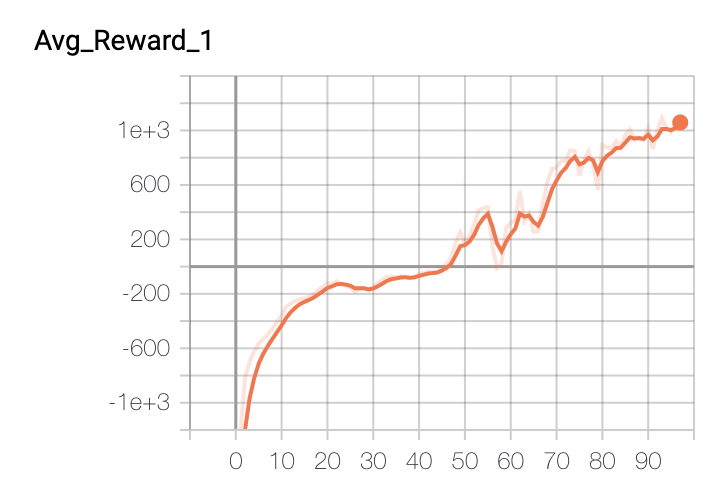
\includegraphics[scale=0.5]{images/cheetah_baseline_12345456_avg_reward.png} \\
  Cheetah no baseline, $r\_seed=12345456$: \\
  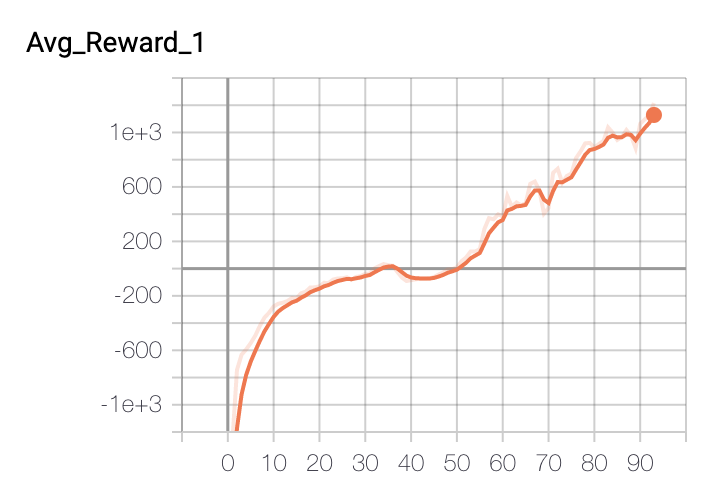
\includegraphics[scale=0.5]{images/cheetah_nobaseline_12345456_avg_reward.png} \\
  Cheetah combined performance: \\  
  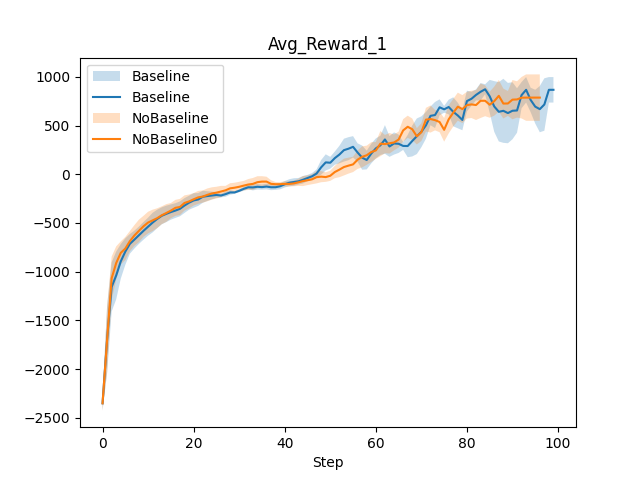
\includegraphics[scale=0.5]{images/cheetah_Avg_Reward_1_combined.png} \\
  The no baseline cases have lower variance across the three random seeds.  There is a bunch of randomness in the environment but it is surprising to see this result happen so consistently.  
  
  \section{Best Arm Identification in Multi-Armed Bandit}
  \paragraph{(a)}    
  As stated in the problem, by Hoeffding's inequality: \\
  $\Pr\bigg{(}|\hat{X}-\bar{X}| > \sqrt{\dfrac{log(2/\delta)}{2n_e}}\bigg{)} < \delta$ \\
  So $\Pr\bigg{(}|\hat{r}_a-\bar{r}_a| \leq \sqrt{\dfrac{log(2/\delta)}{2n_e}}\bigg{)} \geq 1-\delta$ \\
  For each arm this is an independent probability so we can multiply events to get the joint probability: \\
  $\Pr\bigg{(}\forall a \in \mathcal{A}, |\hat{r}_a-\bar{r}_a| \leq \sqrt{\dfrac{log(2/\delta)}{2n_e}}\bigg{)} \geq (1-\delta)^{|\mathcal{A}|}$ \\
  Therefore: \\
  $\Pr\bigg{(}\exists a \in \mathcal{A} \textrm{ s.t. } |\hat{r}_a-\bar{r}_a| > \sqrt{\dfrac{log(2/\delta)}{2n_e}}\bigg{)} < 1-(1-\delta)^{|\mathcal{A}|} \leq |\mathcal{A}|\delta$ \\
  Where the last inequality holds in the problem since $\delta > 0, |\mathcal{A}| >= 1$\\
  \paragraph{ (b) }
  The most difficult case is where the suboptimal $|\mathcal{A}|-1$ arms all have mean $\bar{r}_a=\bar{r}_{a^*}-\epsilon$. \\
  If all arms differ from their actual mean by at most $\dfrac{\epsilon}{2}$ we will be all set.
  Based on the result from part (a), \\
  $\Pr\bigg{(}\exists a \in \mathcal{A} \textrm{ s.t. } |\hat{r}_a-\bar{r}_a| > \sqrt{\dfrac{log(2/\delta)}{2n_e}}\bigg{)} < |\mathcal{A}|\delta$ \\
  We only care about the difference in one direction since the optimal arm's observed mean can't be too low and all other arms' means can't be too high.  Therefore in our case the relevant formula is: \\
  $\Pr\bigg{(}\exists a \in \mathcal{A} \textrm{ s.t. } \hat{r}_a-\bar{r}_a > \sqrt{\dfrac{log(2/\delta)}{2n_e}}\bigg{)} < \dfrac{|\mathcal{A}|\delta}{2}$ \\    
  So in our case let $\delta'=\dfrac{|\mathcal{A}|\delta}{2}$, so $\delta=\dfrac{2\delta'}{|\mathcal{A}|}$.  Then, \\
  $\dfrac{\epsilon}{2} > \sqrt{\dfrac{log(\dfrac{|\mathcal{A}|}{\delta'})}{2n_e}}$ \\
  $\dfrac{\epsilon^2}{4} > \dfrac{log(\dfrac{|\mathcal{A}|}{\delta'})}{2n_e}$ \\
  Then, \\
  $n_e > \dfrac{2log(\dfrac{|\mathcal{A}|}{\delta'})}{\epsilon^2}$
  

\end{document}